\documentclass[border=10pt]{standalone}
\usepackage{pgfplots}
\pgfplotsset{compat=1.18}
\usetikzlibrary{arrows.meta}
\begin{document}
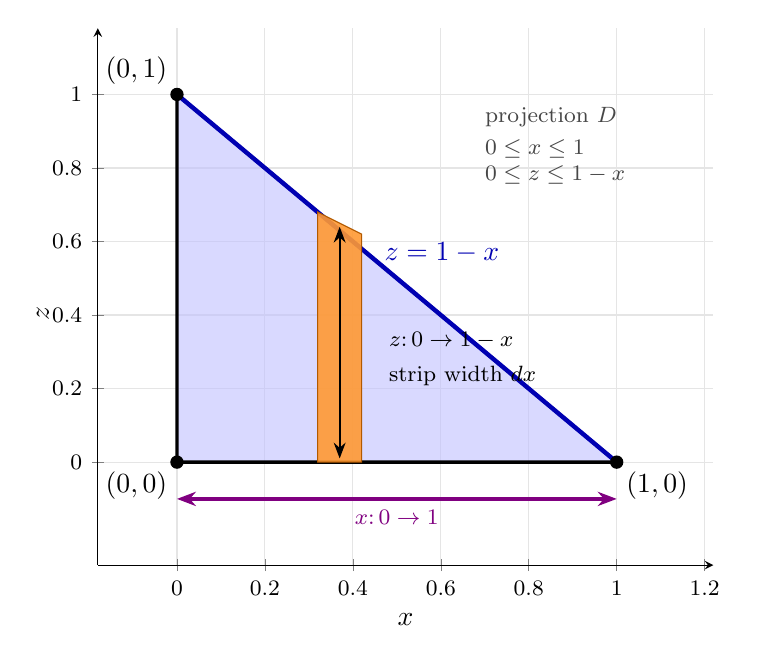
\begin{tikzpicture}
\begin{axis}[
    width=9.4cm, height=8.4cm,
    xmin=-0.18, xmax=1.22, ymin=-0.28, ymax=1.18,
    xtick={0,0.2,...,1.2}, ytick={0,0.2,...,1.0},
    tick label style={font=\footnotesize},
    xlabel=$x$, ylabel=$z$, xlabel style={below}, ylabel style={left},
    grid=major, grid style={gray!20}, clip=false, axis lines=left,
    every node/.style={font=\small},
]
% ---- projection triangle D ----
\addplot[fill=blue!25, fill opacity=.6, draw=black, very thick] coordinates {(0,0) (1,0) (0,1)} -- cycle;
% ---- hypotenuse z = 1-x highlighted ----
\addplot[blue!70!black, line width=1.6pt] coordinates {(0,1) (1,0)};
\node[blue!70!black, right] at (axis cs:0.45,0.57) {$z=1-x$};

% ---- typical vertical strip of width dx ----
\addplot[draw=orange!70!black, fill=orange!80, fill opacity=.9] coordinates {(0.32,0) (0.42,0) (0.42,0.62) (0.32,0.68)} -- cycle;
\draw[{Stealth[length=2mm]}-{Stealth[length=2mm]}, thick, black] (axis cs:0.37,0.01) -- (axis cs:0.37,0.64);
\node[right, align=left, font=\footnotesize] at (axis cs:0.46,0.28) {$z\colon 0\to 1-x$\\[3pt] strip width $dx$};

% ---- x range ----
\draw[{Stealth[length=2.4mm]}-{Stealth[length=2.4mm]}, very thick, violet] (axis cs:0,-0.10) -- (axis cs:1,-0.10);
\node[violet, below, font=\footnotesize] at (axis cs:0.5,-0.105) {$x\colon 0\to 1$};

% ---- corner dots and labels ----
\addplot[only marks, mark=*, mark size=2.2pt, black] coordinates {(0,0) (1,0) (0,1)};
\node[below left]  at (axis cs:0,0) {$(0,0)$};
\node[below right] at (axis cs:1,0) {$(1,0)$};
\node[above left]  at (axis cs:0,1) {$(0,1)$};

\node[align=left, font=\footnotesize, black!72] at (axis cs:0.86,0.86)
     {projection $D$\\[2pt] $0\le x\le 1$\\ $0\le z\le 1-x$};
\end{axis}
\end{tikzpicture}
\end{document}